\chapter{Argumentación}\label{chapter:argumentation}

% Argumentacion background

\section{Argumentación}

% TODO Ampliar esto, basarse en el articulo de MIT \cite{lawrence2020argument}

La argumentación es el proceso que consiste en producir elementos que justifiquen una afirmación. Una afirmación 
constituye una expresión de algo ocurrido, un juicio, una evaluación. Las premisas son los elementos que 
justifican o atacan las afirmaciones. Un argumento básico está dado por la relación entre una afirmación y una 
premisa, con dicha premisa estar atacando o apoyando la afirmación inicial. Un ejemplo básico constituye:

\begin{adjustwidth}{25pt}{25pt}
    \emph{Las vacunas previenen la diseminación de enfermedades}, por lo tanto \textbf{vacunarse es necesario}.
\end{adjustwidth}

En el ejemplo se puede observar un argumento simple y algunas características propias de estos, la justificación 
(en \textbf{negro}) que apoya la afirmación (en \emph{itálico}), también se puede observar palabras conectoras 
que indican además de conexión la dirección de esta.

Sobre esta han surgido diferentes marcos teóricos que buscan una metodología para su representación y estudio. 
Una de las más citadas constituye el Método o Modelo de Toulmin.

El Método Toulmin fue extrapolado del libro \emph{The Uses of Argument} [\cite{toulmin_2003}] escrito por Stephen E. Toulmin.
Este método divide los argumentos en seis partes: afirmación (claim), fundamento (grounds), 
justificación (warrant), calificador (qualifier), refutación (rebuttal) y respaldo (backing).
Mediante las afirmaciones se conoce el argumento principal que el autor quiere probar a la audiencia,
estas son respaldados con fundamentos siendo estos las evidencias y hechos en que se apoya el autor.
Las justificaciones pueden estar explícitas o implícitas y son suposiciones que vinculan los
fundamentos con las afirmaciones, estas a su vez pueden ser respaldadas por conocimiento.
El esquema introduce la posibilidad de otra sitaución válida a la establecida en las afirmaciones
mediante la refutación. Los calificadores son usados para dar más información de la calidad o seguridad
de las afirmaciones dadas. Un ejemplo de este esquema es:

\begin{adjustwidth}{25pt}{25pt}
    [\emph{Se escucharon ladridos y aullidos en la distancia}]$_{fundamento}$, 
    [\emph{probablemente}]$_{calificador}$ 
    [\emph{haya perros en las cercanías}]$_{afirmación}$.
\end{adjustwidth}

En este ejemplo, además de las partes explícitas, se encuentran implícitas como la justificación 
(los perros son animales que ladran y aullan), el respaldo (se sabe que existen perros en la zona) y 
la refutación (Puede ser que hayan lobos o coyotes cerca). [\cite{toulminArgument}]
  
\section{Extracción de Argumentos}

El Procesamiento de Lenguaje Natural (\textbf{NLP} por sus siglas en inlgés \emph{Natural Language Processing}) es un 
subcampo de la Inteligencia Artificial (IA) que tiene como objetivo la comprensión del lenguaje humano por 
las computadoras. 
Mediante el uso de sus algoritmos es posible el procesamiento masivo de texto para la extracción de información 
relvante de este. Entre las tareas pertenecientes a dicho campo se encuentran Traducción Automática, 
Generación de Lenguaje Natural y Extracción de Argumentos (EA). La EA constituye la identificación y extracción 
automática de las estructuras de inferencia y 
razonamiento expresadas como argumentos presentes en el lenguaje natural [\cite{lawrence2020argument}].
En la actualidad en tareas de \textbf{NLP} como análisis de sentimientos permiten 
extraer cuales son las opiniones o sentimientos presentes, este análisis, sin embargo, presenta una falta 
de información, ya que no presenta el porqué de estas. La EA permite dar respuesta a este problema presentando
los argumentos y cómo sus relaciones justifican sus posiciones.

\subsection{Estructuras Argumentativas}

% TODO HAblar de esquemas argumentativos? Esto seria las clasificaiones seleccionadas para las UDA y relaciones
% además del método para segmentación de UDA y el criterio de marcar las relaciones

Las estructuras argumentativas son las partes y sus relaciones de las cuales están compuestas la argumentación en los textos.
Estas se componen de dos elementos principales, las Unidades de Discurso Argumentativas (UDA) y los enlaces
existentes entre estas. Las UDAs presentan varias definiciones en las que se ven como cláusulas, oraciones, aunque
todas estas se presentan como secciones consecutivas de texto que no se sobreponen. Estas UDAs se relacionan entre 
sí formando el proceso de inferencia y razonamiento.
Tanto los enlaces como las UDAs son clasificadas en dependencia de su rol en la argumentación, estas clasificaciones 
parten de los conceptos de premisa y afirmación para las UDA y ataque y apoyo para las relaciones. 

\subsection{Tareas de extracción de argumentos}

Dada las estructuras argumentativas en la EA se conciben las siguientes tareas principales:

\subsubsection{Extracción de UDAs}

Esta tarea constituye en la separación de los segmentos de texto que formarán parte de la estructura.
El texto entrado es segmentado y como salida se obtiene un conjunto de UDAs. En el siguiente ejemplo se 
pone un ejemplo de la extracción de UDAs (en \emph{itálico}).

\begin{adjustwidth}{25pt}{25pt}
    Existen muchos efectos de la expansión de la tecnología en la transportación y las comunicaciones,
    las cuales son mencionanadas ahora. En primer lugar, [\emph{el correo electronico puede contar como uno de los resultados
    más beneficiosos de la tecnología moderna}]. [\emph{Años atrás, las personas pagaban gran cantidad de dinero para 
    enviar sus cartas y sus pagos estaban sujetos al peso de sus cartas o paquetes y muchos accidentes podrían 
    causar problemas que causarían que el correo no fuera enviado}].
\end{adjustwidth}

\subsubsection{Clasificación de UDAs}

La clasificación de UDAs consiste en asignarle el papel que toma la UDA en la argumentación. En general 
las clasificaciones parten de dos clases bases, las afirmaciones, las cuales son posiciones que toma el 
autor del texto y las premisas, que son datos, eventos, elementos que se consideran verdades por sí solas.  

\begin{adjustwidth}{25pt}{25pt}
    Existen muchos efectos de la expansión de la tecnología en la transportación y las comunicaciones, 
    las cuales son mencionanadas ahora. En primer lugar, [\emph{el correo electronico puede contar como uno de los resultados
    más beneficiosos de la tecnología moderna}]$_{Afirmación}$. [\emph{Años atrás, las personas pagaban gran cantidad de dinero para 
    enviar sus cartas y sus pagos estaban sujetos al peso de sus cartas o paquetes y muchos accidentes podrían 
    causar problemas que causarían que el correo no fuera enviado}]$_{Premisa}$.
\end{adjustwidth}

\subsubsection{Extracción de relaciones entre las UDAs}

La extracción de relaciones constituye en determinar si estan relacionadas las UDAs. La disposición de estas
relaciones forma el proceso de razonamiento en que se basa el autor para validar su posición. En el ejemplo 
se representa la existencia de relación mediante su distancia argumentativa con la UDA con la que se relaciona.
La distancia argumentativa son la cantidad de UDAs del texto que separan la UDA fuente del objetivo [\cite{galassi2018argumentative}], 
en caso de ser negativa el objetivo se encuentra antes que la fuente y viceversa.

\begin{adjustwidth}{25pt}{25pt}
    Existen muchos efectos de la expansión de la tecnología en la transportación y las comunicaciones, 
    las cuales son mencionanadas ahora. En primer lugar, [\emph{el correo electronico puede contar como uno de los resultados
    más beneficiosos de la tecnología moderna}]$_{Afirmación}$. [\emph{Años atrás, las personas pagaban gran cantidad de dinero para 
    enviar sus cartas y sus pagos estaban sujetos al peso de sus cartas o paquetes y muchos accidentes podrían 
    causar problemas que causarían que el correo no fuera enviado}]$_{Premisa, -1}$.
\end{adjustwidth}

\subsubsection{Clasificación de relaciones entre las UDAs}

Los tipos de relaciones, nacen de dos clases bases por lo general, están las relaciones de apoyo y las de ataque.
Las de apoyo se centran en aquellas en las que la UDA fuente afirme la UDA objetivo, las de ataque se basan en 
las que la UDA fuente apoye la negación de la UDA objetivo.

\begin{adjustwidth}{25pt}{25pt}
    Existen muchos efectos de la expansión de la tecnología en la transportación y las comunicaciones, 
    las cuales son mencionanadas ahora. En primer lugar, [\emph{el correo electronico puede contar como uno de los resultados
    más beneficiosos de la tecnología moderna}]$_{Afirmación}$. [\emph{Años atrás, las personas pagaban gran cantidad de dinero para 
    enviar sus cartas y sus pagos estaban sujetos al peso de sus cartas o paquetes y muchos accidentes podrían 
    causar problemas que causarían que el correo no fuera enviado}]$_{Premisa, -1, apoyo}$.
\end{adjustwidth}

Partiendo de esto, se puede observar que las estructuras argumentativas de un texto constituyen un grafo dirigido 
en donde sus nodos representan las UDA y están anotados con su tipo y sus vértices representan las 
relaciones entre las UDA y dichos vértices se anotan con el tipo de relación existente entra ambas (\ref{fig:arg_struct}).

\begin{figure}[h!]
	\begin{center}
		\begin{center}
			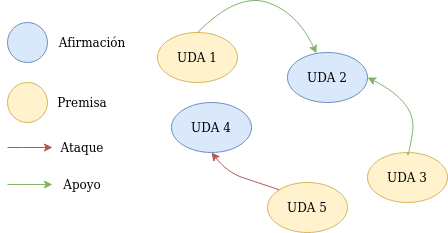
\includegraphics[scale=.7]{Graphics/Estructuras_argumentativas.png}
            % \includesvg[options]{Graphics/Estructuras argumentativas.svg}
        \end{center}
	    \caption{Estructuras Argumentativas}
	\end{center}
\end{figure}\label{fig:arg_struct}
